\chapter{Integral Kalkulus}

\section*{Pengantar}

Pada Bab~2, kita telah mempelajari sifat-sifat fungsi secara umum. Pada bab ini, kita mempelajari bagaimana menghitung \textbf{laju perubahan} fungsi (kalkulus diferensial) dan \textbf{luasan di bawah kurva} fungsi (kalkulus integral). Kalkulus diferensial dan integral merupakan dua sisi dari satu koin yang sama; keduanya dihubungkan oleh \textbf{Teorema Dasar Kalkulus}. Penguasaan kalkulus sangat penting karena menjadi landasan bagi hampir semua analisis dalam matematika rekayasa, termasuk Deret Fourier (Bab~6) yang melibatkan integral untuk menghitung koefisien, dan Analisa Sistem (Bab~7) yang menggunakan integral konvolusi.

\section{Kalkulus Diferensial}
Fenomena fisis seringkali berurusan dengan sesuatu yang berubah terhadap waktu atau dengan kata lain berubah secara kontinu. Matematika kalkulus digunakan untuk berurusan dengan hal-hal yang berkenaan dengan perubahan kontinu. Kalkulus berhubungan dengan limit. Untuk memahami ide tentang limit, bayangkan kita memiliki urutan bilangan $l_1, l_2, l_3,\ldots$ yang nilainya semakin dekat dengan sebuah nilai $L$. Sebagai contoh: $0{,}9;\; 0{,}99;\; 0{,}999;\; 0{,}9999;\;\ldots$ Dapat dikatakan bahwa limit dari urutan ini sama dengan 1. Tidak ada satu pun dari angka-angka tersebut yang sama dengan 1, akan tetapi semakin lama semakin mendekati nilai 1. Jika ide ini digunakan pada fungsi yang berubah sejalan dengan waktu $f(t)$, maka $L$ adalah limit dari fungsi ketika $t$ mendekati nilai tertentu, misalnya $a$:
\begin{equation}
\lim_{t\rightarrow a}f(t)=L.
\end{equation}

Kalkulus diferensial berhubungan dengan laju perubahan fungsi $\Delta f$ terhadap perubahan waktu $\Delta t$. Sepanjang interval $\Delta t$, fungsi berubah dari $f(t)$ menjadi $f(t+\Delta t)$, sehingga
\begin{equation}
\Delta f = f(t+\Delta t) - f(t).
\end{equation}

\begin{figure}[!h]
\centering
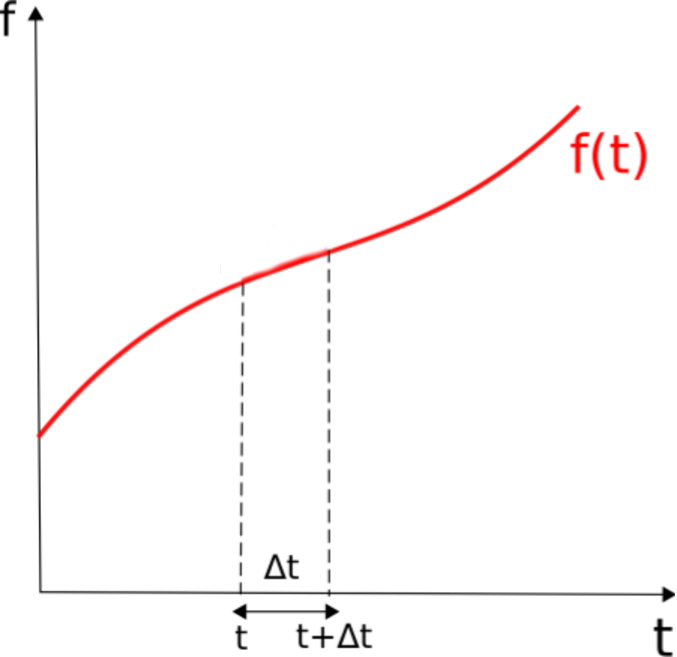
\includegraphics[scale=0.6]{pict/differentialgraph.pdf}
\caption{Grafik fungsi yang berubah terhadap waktu; $\Delta f$ menunjukkan perubahan fungsi, $\Delta t$ menunjukkan perubahan waktu}\label{fig:differential}
\end{figure}

Untuk mendefinisikan laju perubahan pada satu saat $t$ secara akurat, kita harus menyusutkan $\Delta t$ sampai nol. Jika kita membagi $\Delta f$ dengan $\Delta t$ dan mengambil limit, kita memperoleh \textbf{turunan} (\textit{derivatif}) dari fungsi $f(t)$ terhadap waktu $t$:
\begin{equation}
\frac{df}{dt}=\lim_{\Delta t \rightarrow 0} \frac{\Delta f}{\Delta t}=\lim_{\Delta t \rightarrow 0} \frac{f(t + \Delta t)-f(t)}{\Delta t}.
\end{equation}

\begin{exmp}
Hitunglah turunan dari $f(t) = t^2$!

\textbf{Penyelesaian:}\\
\begin{align*}
f(t+\Delta t) &= (t+\Delta t)^2 = t^2 + 2t\Delta t + \Delta t^2. \\
\frac{f(t+\Delta t) - f(t)}{\Delta t} &= \frac{2t\Delta t + \Delta t^2}{\Delta t} = 2t + \Delta t. \\
\frac{df}{dt} &= \lim_{\Delta t\to 0}(2t + \Delta t) = 2t.
\end{align*}
\end{exmp}

Dengan menggunakan \textbf{teorema binomial}, dapat ditunjukkan bahwa untuk fungsi perpangkatan umum $f(t) = t^n$, berlaku:
\begin{equation}
\frac{d(t^n)}{dt}=nt^{n-1},
\end{equation}
untuk sembarang bilangan real $n$.

\subsection{Aturan-aturan Turunan}

\begin{enumerate}
\item \textbf{Turunan konstanta}: $\dfrac{dc}{dt} = 0$.
\item \textbf{Kelipatan konstanta}: $\dfrac{d(cf)}{dt} = c\,\dfrac{df}{dt}$.
\item \textbf{Aturan penjumlahan}: $\dfrac{d(f+g)}{dt} = \dfrac{df}{dt} + \dfrac{dg}{dt}$.
\item \textbf{Aturan hasil kali}: $\dfrac{d(fg)}{dt} = f\,\dfrac{dg}{dt} + g\,\dfrac{df}{dt}$.
\item \textbf{Aturan rantai}: Jika $f = f(g)$ dan $g = g(t)$, maka $\dfrac{df}{dt} = \dfrac{df}{dg}\cdot\dfrac{dg}{dt}$.
\end{enumerate}

\begin{exmp}
Hitunglah turunan dari $f(t) = \ln t^3$ menggunakan aturan rantai!

\textbf{Penyelesaian:}\\
Ambil $g = t^3$ sehingga $f(g) = \ln g$. Maka:
\[
\frac{df}{dt} = \frac{df}{dg}\cdot\frac{dg}{dt} = \frac{1}{g}\cdot 3t^2 = \frac{3t^2}{t^3} = \frac{3}{t}.
\]
\end{exmp}

\section{Kalkulus Integral}

Jika kalkulus diferensial berhubungan dengan \textit{laju perubahan}, kalkulus integral berhubungan dengan \textit{penjumlahan bagian-bagian kecil}. Masalah utamanya adalah menghitung luasan di bawah kurva yang didefinisikan oleh fungsi $f(t)$.

\begin{figure}[!h]
\centering
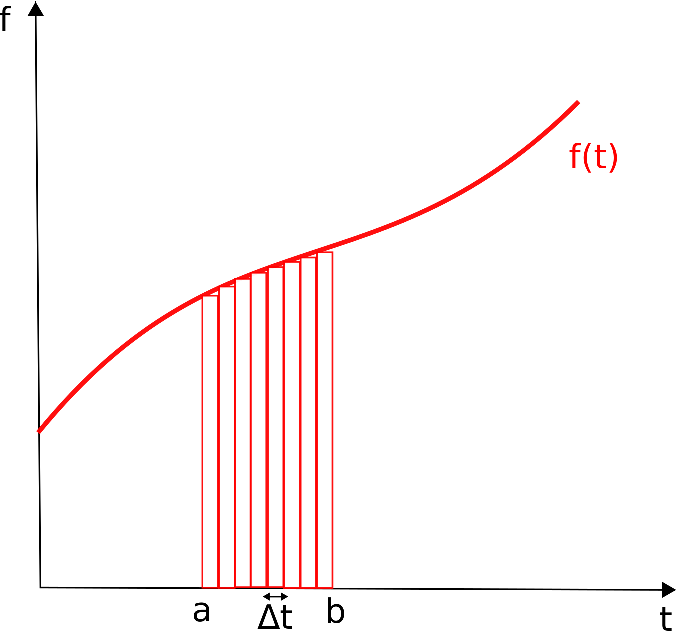
\includegraphics[scale=0.6]{pict/integralgraph-eps-converted-to.pdf}
\caption{Luasan di bawah kurva $f(t)$ didekati dengan penjumlahan persegi panjang}\label{fig:integral}
\end{figure}

Luasan sebuah persegi panjang kecil adalah $\delta A = f(t)\,\Delta t$. Jumlahan seluruhnya:
\[
A = \sum_{i}^{N} f(t_i)\,\Delta t.
\]
Dengan menyusutkan $\Delta t \to 0$ dan $N \to \infty$, diperoleh \textbf{integral tertentu}:
\begin{equation}
A = \int_a^b f(t)\,dt = \lim_{\Delta t \to 0}\sum_i f(t_i)\,\Delta t.
\end{equation}

Integral tak tentu direpresentasikan sebagai fungsi $F(t)$:
\begin{equation}
F(t) = \int f(t)\,dt.
\end{equation}

Hubungan antara integral dan turunan bersifat resiprokal (Teorema Dasar Kalkulus):
\[
\frac{dF}{dt} = f(t).
\]

Untuk fungsi perpangkatan $f(t) = t^n$:
\begin{equation}
\int t^n\,dt = \frac{t^{n+1}}{n+1} + C, \quad n \ne -1.
\end{equation}

\textbf{Teorema Dasar Kalkulus} secara umum:
\begin{equation}
\int_a^b f(t)\,dt = F(b) - F(a).
\end{equation}

\subsection{Rumus-rumus Integrasi}

\begin{itemize}
\item $\displaystyle\int c\,dt = ct + C$
\item $\displaystyle\int cf(t)\,dt = c\int f(t)\,dt$
\item $\displaystyle\int t^n\,dt = \dfrac{t^{n+1}}{n+1} + C \quad (n \ne -1)$
\item $\displaystyle\int \sin t\,dt = -\cos t + C$
\item $\displaystyle\int \cos t\,dt = \sin t + C$
\item $\displaystyle\int e^t\,dt = e^t + C$
\item $\displaystyle\int \frac{dt}{t} = \ln|t| + C$
\item $\displaystyle\int [f(t) \pm g(t)]\,dt = \int f(t)\,dt \pm \int g(t)\,dt$
\end{itemize}

\subsection{Integrasi Parsial}

Integrasi parsial merupakan kebalikan dari aturan hasil kali turunan. Jika $u = f(x)$ dan $v = g(x)$, maka:
\begin{equation}
\int u\,dv = uv - \int v\,du.
\end{equation}

\begin{exmp}
Hitunglah $\displaystyle\int_0^{\pi/2} x\cos x\,dx$!

\textbf{Penyelesaian:}\\
Ambil $v = x$ ($dv = dx$) dan $du = \cos x\,dx$ ($u = \sin x$). Maka:
\begin{align*}
\int_0^{\pi/2} x\cos x\,dx &= x\sin x\Big|_0^{\pi/2} - \int_0^{\pi/2}\sin x\,dx \\
&= \frac{\pi}{2}\sin\frac{\pi}{2} + \cos x\Big|_0^{\pi/2} \\
&= \frac{\pi}{2} + (0 - 1) = \frac{\pi}{2} - 1.
\end{align*}
\end{exmp}

\section*{Rangkuman}

Pada bab ini telah dibahas dua pilar utama kalkulus. \textbf{Kalkulus diferensial} menghitung laju perubahan fungsi melalui limit dan menghasilkan turunan. \textbf{Kalkulus integral} menghitung luasan di bawah kurva melalui penjumlahan tak berhingga dan menghasilkan integral. Kedua operasi ini saling invers melalui Teorema Dasar Kalkulus: $dF/dt = f(t)$.

Aturan-aturan turunan (aturan penjumlahan, aturan hasil kali, aturan rantai) dan teknik integrasi (integrasi langsung, integrasi parsial) merupakan alat utama dalam matematika rekayasa. Kalkulus integral akan banyak digunakan pada Bab~6 untuk menghitung koefisien Fourier, dan pada Bab~7 untuk menghitung konvolusi.

\section*{Latihan Soal}

\begin{enumerate}
  \item Hitunglah turunan dari fungsi-fungsi berikut:
  \begin{enumerate}[(a)]
    \item $f(t) = 3t^4 - 2t^2 + 7$
    \item $f(t) = \sin(t^2)$
    \item $f(t) = e^{-t}\cos t$
  \end{enumerate}
  \item Hitunglah integral-integral berikut:
  \begin{enumerate}[(a)]
    \item $\displaystyle\int (3x^2 + 2x - 1)\,dx$
    \item $\displaystyle\int_0^1 e^{2x}\,dx$
    \item $\displaystyle\int x\,e^x\,dx$ \quad (gunakan integrasi parsial)
  \end{enumerate}
  \item Gunakan aturan rantai untuk menghitung $\dfrac{dy}{dx}$ jika $y = \sqrt{1 + x^2}$!
  \item Tunjukkan bahwa $\displaystyle\int_0^T \sin(n\omega_0 t)\,dt = 0$ jika $T = 2\pi/\omega_0$ dan $n$ bilangan bulat!
\end{enumerate}



